\chapter{Proposta de trabalho}

\textit{Blockchain} se tornou um assunto recorrente nos últimos anos. O assunto tem se tornado relevante, tanto pela adoção massiva em criptomoedas, como pelo recente interesse do sistema financeiro tradicional. Em movimento inédito a China tem testado uma versão digital do Yuan \cite{Carvalho2020}. O interesse chegou também ao Brasil e o Banco Central tem ventilado a possibilidade de um Real Digital, baseado em DLT \cite{Tecmundo2021}.

As tendências de agregar a tecnologia aos sistemas de votação existente também tem ganhado momento. Trabalhos como \citeonline{Patidar2019}, \citeonline{Mpekoa2017}, \citeonline{Ahmed2020}, \citeonline{Bistarelli2019} e \citeonline{Yi2019} tem demonstrado a tendência da comunidade acadêmica quanto ao uso das tecnologias aqui discutidas. O interesse também foi despertado o interesse do TSE \cite{GUSSON}. 

A proposta deste trabalho, a fim de testar hipótese apresentada, seria o desenvolvimento de provas de conceito, com base em um protocolo desenhado para comunicação entre nós e testes públicos, entretanto a abordagem foi dificultada pela pandemia mundial de COVID-19. Assim sendo, a fim de dar prosseguimento a testagem da hipótese, dois aplicativos, detalhados adiante, foram desenvolvidos e testados, a fim de aferir a hipótese deste trabalho. 

As aplicações de coleta de dados, identificação dos usuários e coleta de voto deverão rodar sobre um computador \gls{sbc1} \gls{rpi} 4, que executa uma distribuição Linux específica para arquitetura ARM64, que por sua vez vai executar o interpretador da linguagem Python. 

\begin{figure}[h!]
	\centering
	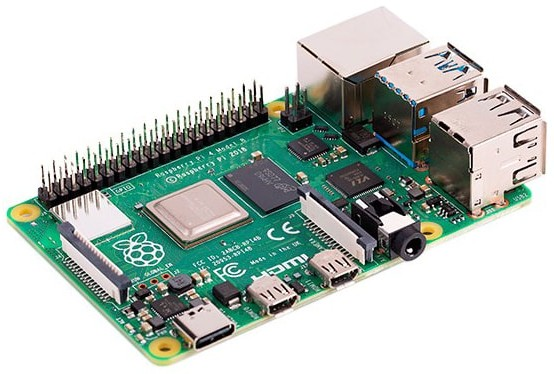
\includegraphics[width=0.6\textwidth]{imagens/rpi4}
	\caption{Placa SBC Raspberry Pi 4}
	\label{fig:rpi4}
\end{figure}
